% Author: Ben Champion <bwc3252@rit.edu>
% Main LaTeX file for Lenfest Community Weekend 2019 Presentation

\documentclass{beamer}

\usetheme{Amsterdam}

\usepackage{caption}

\begin{document}
\title{Astrophysical Parameter Inference with Gravitational Wave and Electromagnetic Data Channels}
\author{Ben Champion}
\institute{Rochester Institute of Technology \\ Center for Computational Relativity and Gravitation}

% logos
\titlegraphic{
\includegraphics[width=6cm]{Images/RIT_RGB_hor_k}\hspace*{2cm}~%
   
\includegraphics[width=2cm]{Images/ccrg_logo}
}

\date{
  \today
}

\frame{
  \titlepage
}

\frame{ \frametitle{Table of contents}
  \tableofcontents
}

\section{Introduction}

\frame{ \frametitle{Classical Physics}
  \begin{itemize}
    \item Late 1600s - Newton's law of universal gravitation:
    \begin{figure}
      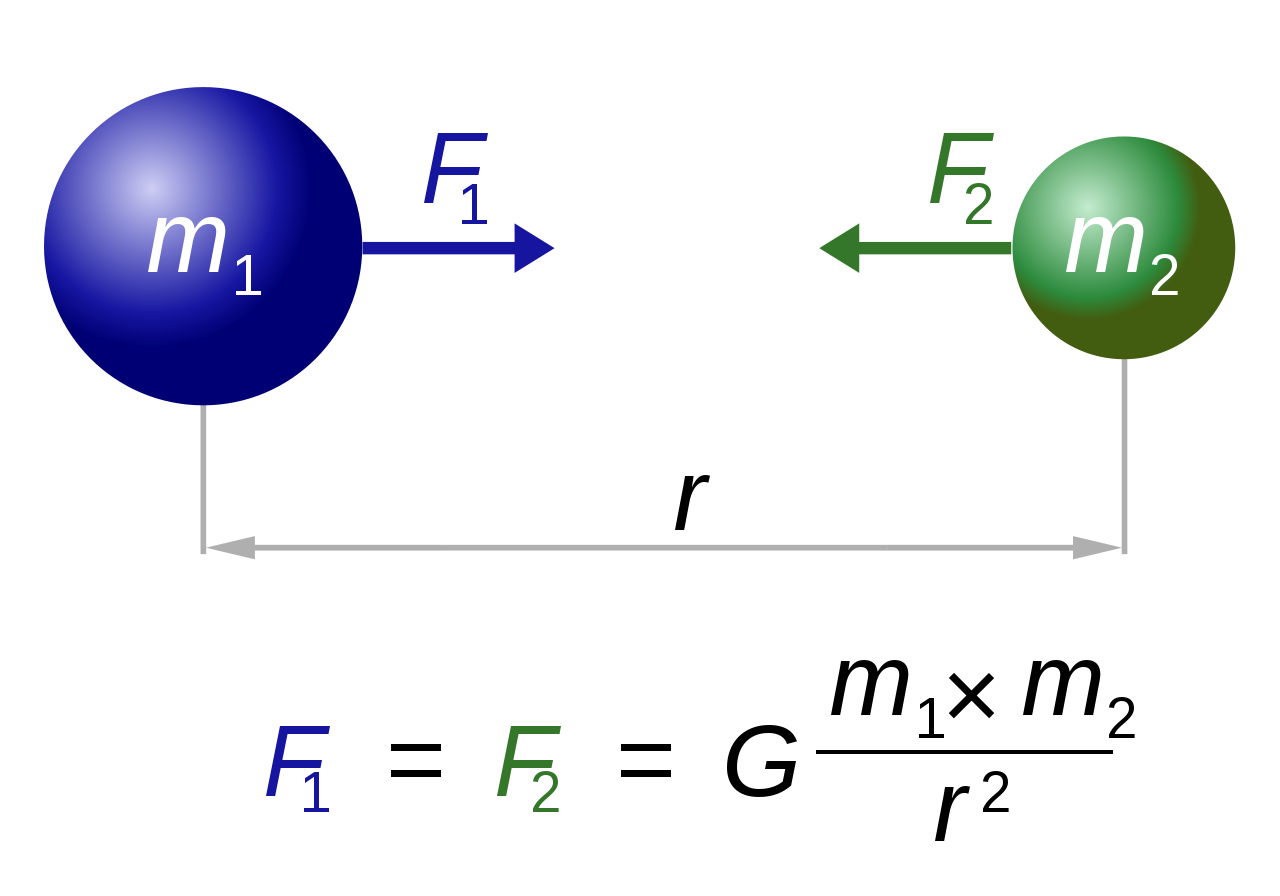
\includegraphics[width=1.75in]{Images/universal_gravitation}
      \caption*{\fontsize{8pt}{10pt}\selectfont Image by Dennis Nilsson}
    \end{figure}
  \end{itemize}
}

\frame{ \frametitle{Special Relativity}
  \begin{columns}[c]
    \column{3.0in}
    \begin{itemize}
      \item 1905 - Einstein's theory of Special Relativity \pause
      \begin{itemize}
        \item The speed of light is independent of the motion of the observer \pause
        \item Consequences include length contraction, time dilation, etc. \pause
        \item Shortcoming: only applies to inertial (non-accelerating) reference frames \pause
      \end{itemize}
    \end{itemize}
    \column{1.5in}
    \begin{figure}
      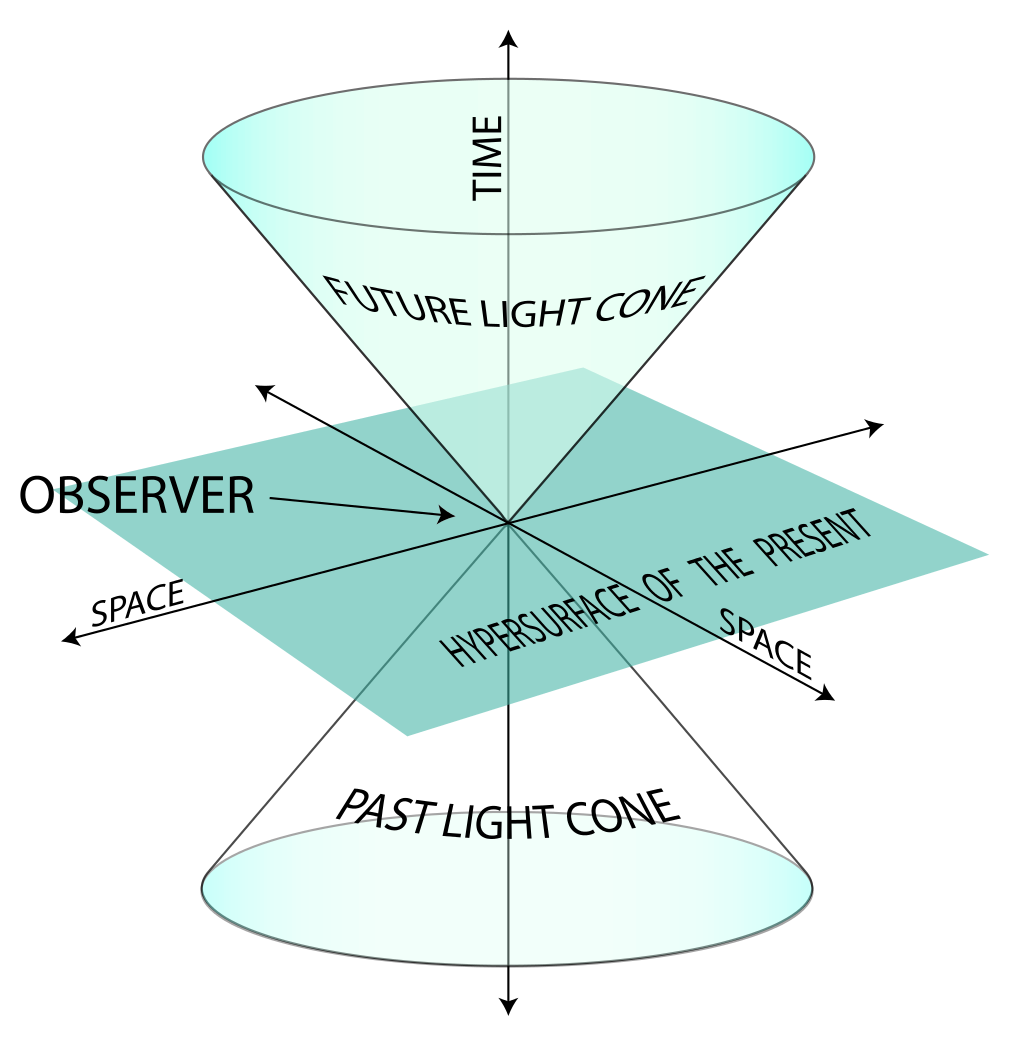
\includegraphics[width=\linewidth]{Images/world_line}
      \caption*{\fontsize{8pt}{10pt}\selectfont Lightcone: the path through spacetime that a single "flash" of light, traveling in all directions, would take (image by K. Aainsqatsi)}
    \end{figure}
  \end{columns}
}

\frame{ \frametitle{Special Relativity}
  Classically, for an event with coordinates $(t, x)$ as measured by a stationary observer and $(t', x')$ as measured by an observer moving with velocity $v$:

  \begin{align*}
    t' &= t  \\
    x' &= x - vt
  \end{align*}

  \pause

  However, according to Special Relativity:

  \begin{align*}
    t' &= \gamma (t - \frac {vx} {c^2}) \\
    x' &= \gamma (x - vt) \\
    \text{where } \gamma &= \frac {1} {\sqrt{1 - \frac {v^2} {c^2}}}
  \end{align*}

  }

\frame{ \frametitle{General Relativity}
  \begin{itemize}
    \item 1915 - Einstein's theory of General Relativity \pause
    \begin{itemize}
      \item Einstein's efforts to include acceleration and external forces (e.g. gravity) in relativity resulted in his theory of General Relativity \pause
      \item Objects with mass change the geometry of spacetime itself \pause
    \end{itemize}
    \item Einstein field equations: describe relationship between four-dimensional spacetime and and the energy-momentum contained in that spacetime \pause \\
    \begin{align*}
      R_{\mu v} - \frac {1} {2} R g_{\mu v} + \Lambda g_{\mu v} = \frac {8 \pi G} {c^4} T_{\mu v}
    \end{align*}
  \end{itemize}
}

\frame{ \frametitle{Einstein Field Equations}
  \begin{columns}[c]
    \column{2.5in}
    \begin{align*}
      R_{\mu \nu} - \frac {1} {2} R g_{\mu \nu} + \Lambda g_{\mu \nu} = \frac {8 \pi G} {c^4} T_{\mu \nu}
    \end{align*}
    \begin{tabular}{l l}
      $R_{\mu v}$   & Ricci curvature tensor \\
      $R$           & scalar curvature \\
      $g_{\mu \nu}$ & metric tensor \\
      $\Lambda$     & cosmological constant \\
      $T_{\mu \nu}$ & stress-energy tensor
    \end{tabular}
    \column{2.0in}
    \begin{figure}
      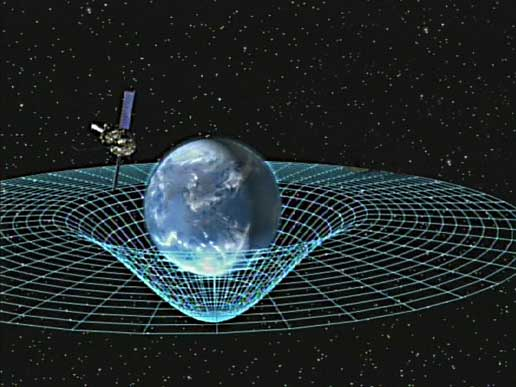
\includegraphics[width=\linewidth]{Images/general_relativity}
    \end{figure}
  \end{columns}
}

\frame{ \frametitle{Gravitational Waves}
  \begin{itemize}
    \item Objects with mass cause distortions in spacetime \pause
    \item Motion involving acceleration produces gravitational waves \pause
    \begin{itemize}
      \item (assuming this motion does not involve spherical or rotational symmetry) \pause
    \end{itemize}
    \item The gravitational waves produced by most objects are too small to detect \pause
    \item Gravitational waves produced by merging black holes or neutron stars are large enough to detect
  \end{itemize}
}

\frame{ \frametitle{Gravitational Wave Interferometry}
  \begin{columns}[c]
    \column{2.5in}
    \begin{itemize}
      \item LIGO - the Laser Interferometer Gravitational Wave Observatory - has two detectors
    \end{itemize}
    \begin{figure}
      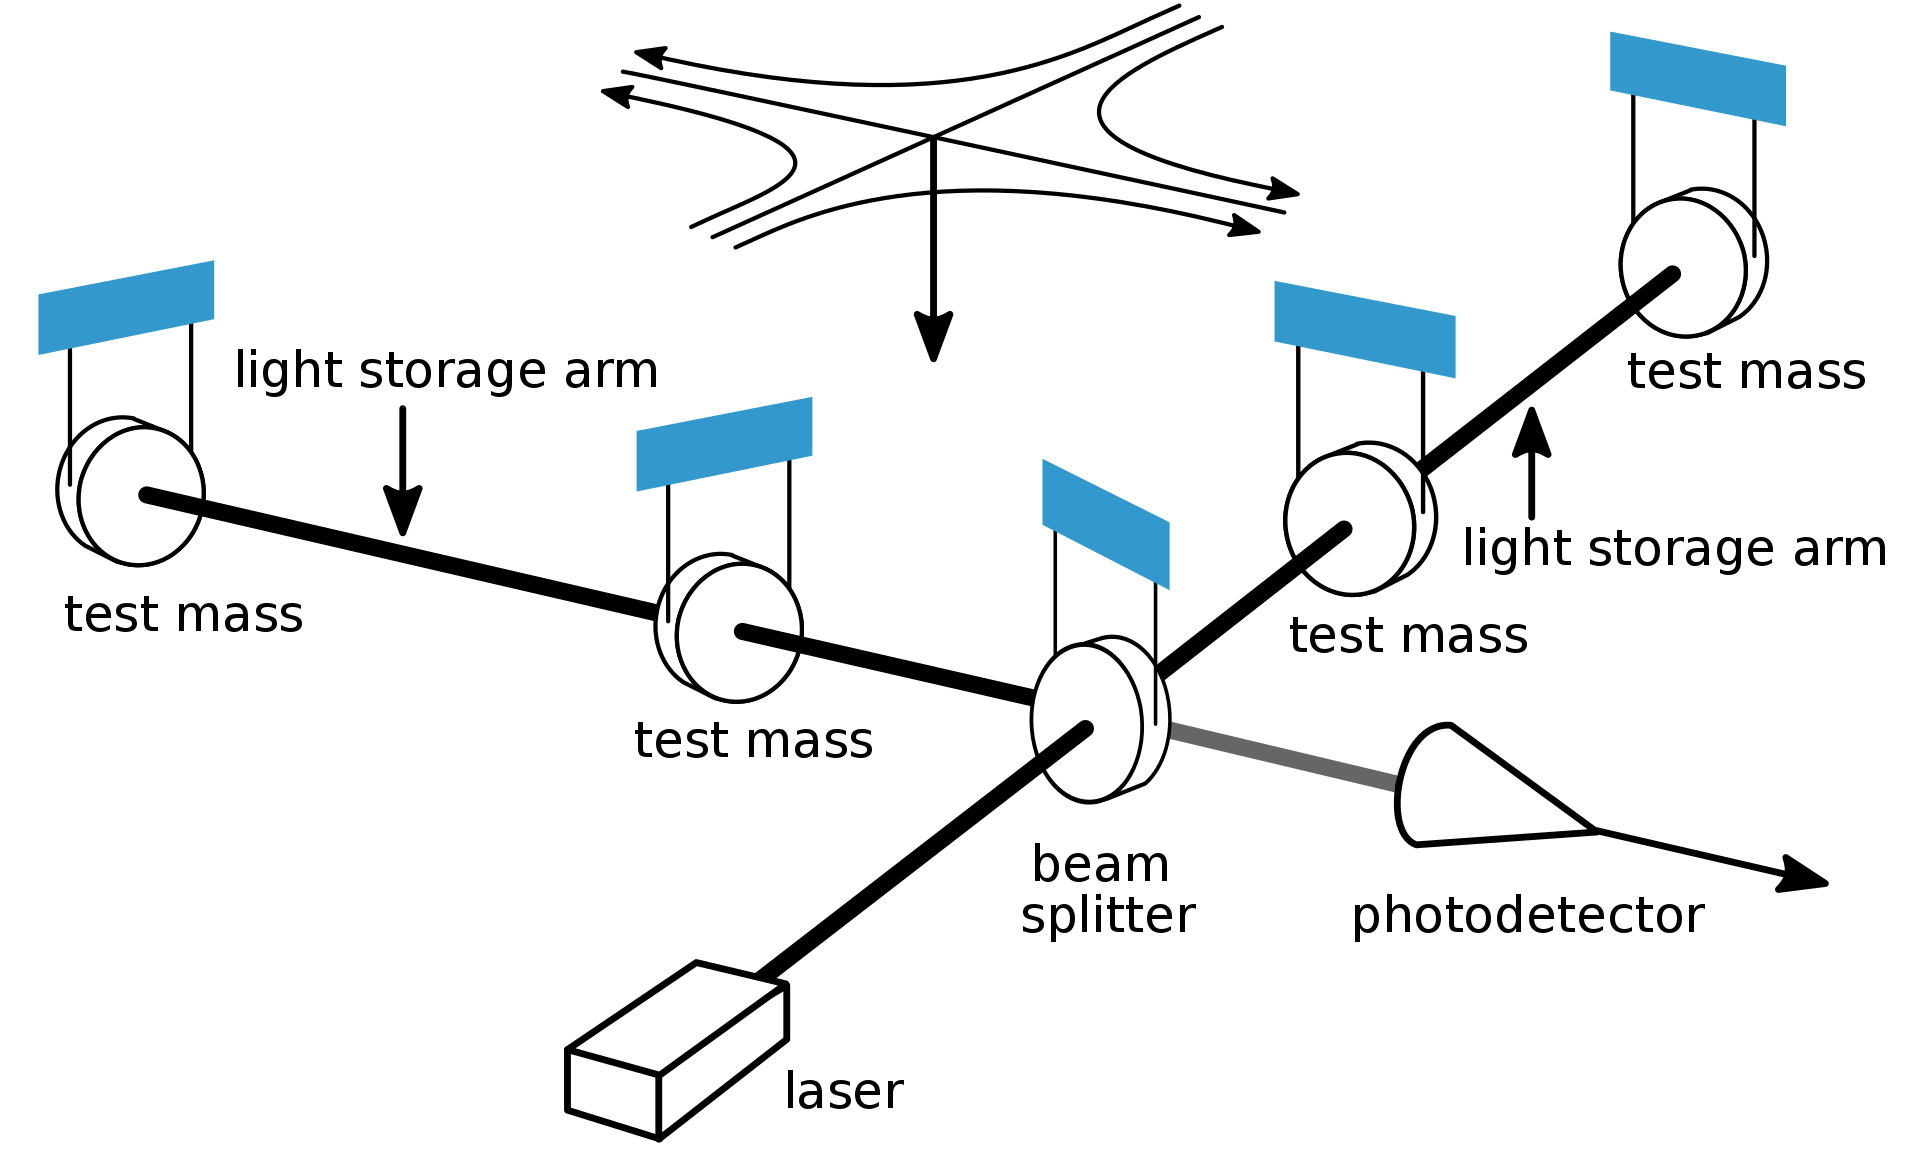
\includegraphics[width=2.0in]{Images/interferometer}
      \caption*{\fontsize{8pt}{10pt}\selectfont Image by Barry Barish}
    \end{figure}
    \pause
    \column{2.25in}
    \begin{itemize}
      \item As a gravitational wave passes, one arm stretches and the other shrinks \pause
      \item When the arms are the same length, the interference pattern detected is completely destructive \pause
      \item When one arm is longer than the other, it takes light more time to travel down that arm, resulting in a detectable interference pattern
    \end{itemize}
  \end{columns}
}

\frame{ \frametitle{Gravitational Wave Detections}
  \begin{figure}
    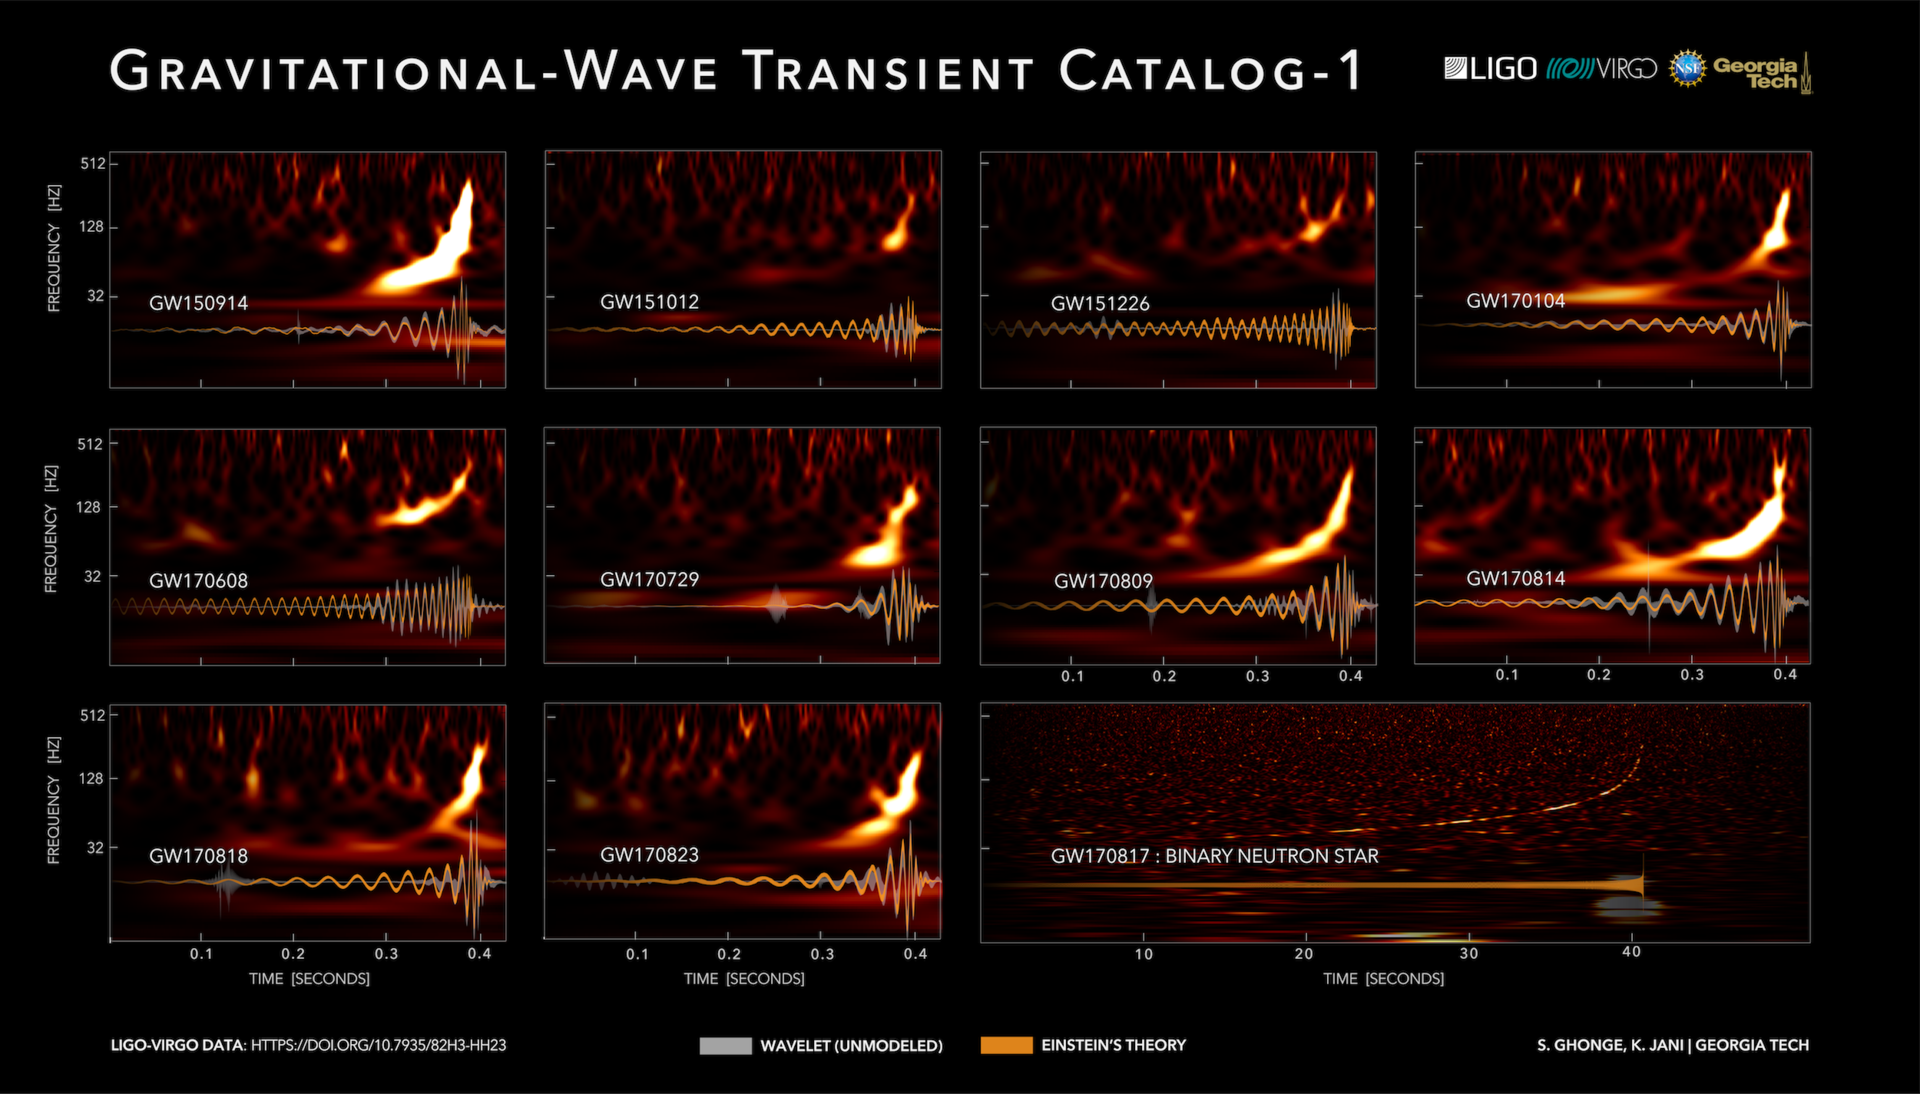
\includegraphics[width=\linewidth]{Images/detections}
    \caption*{\fontsize{8pt}{10pt}\selectfont Image by LIGO/Virgo/Georgia Tech/S. Ghonge \& K. Jani}
  \end{figure}
}

\section{Gravitational Wave PE}

\frame{
}

\section{Neutron Star Mergers and Kilonovae}

\frame{
}

\section{Joint GW/EM PE}

\frame{
}

\section{Results}

\frame{
}

\end{document}
